% !TeX root = ../main.tex

\chapter{Final Project}

\begingroup \linespread{.4}\selectfont
Grading Criteria: Finishing the \textbf{Minimal} parts guarantees 85\% points.
With 1 step solved in \textbf{Advanced} part, you get the rest. Beyond that, you
get bonuses.
\endgroup

\begin{problem}
  Consider the following two-band/orbital Hubbard models at quarter filling on a
  2D lattice.
  \begin{multline*}
    \mathcal H
  = \sum_{ij,\sigma} \sum_{m=1}^2 t_{ij}
    c_{i,\sigma,m}^\dagger c_{j,\sigma,m}
  - \mu \sum_{i,\sigma} \sum_{m=1}^2 n_{i,\sigma,m}
  + U\sum_i \sum_{m=1}^2 n_{i,\uparrow,m} n_{i,\downarrow, m}\\
  - 2J_H \sum_i \vec S_{i,1} \cdot \vec S_{i,2}
  + (U' - J_H/2) \sum_i (n_{i,\uparrow,1} + n_{i,\downarrow,1})
    (n_{i,\uparrow,2} + n_{i,\downarrow,2}).
  \end{multline*}
  Here $i$, $j$ label the lattice sites; $m = 1$, $2$ is the orbital
  and $\sigma$ the spin index. Thus, $c_{i,\sigma,m}^\dagger$ creates an
  electron at site $i$ in orbital $m$ with spin $\sigma$.
  As usual, $\mu$ represents the chemical potential with $n = c^\dagger c$
  being the density operator.

  For simplicity, it is easier to consider the cases for which there are two
  orbitals on each lattice site.

  Brief explanation of the model: $U$ and $U'$ are intra- and inter-orbital
  Coulomb interactions; $J_H$ is the so-called Hund's rule coupling, which is a
  collective result of both Coulomb repulsion and Pauli exclusion principle in
  the atomic states. It is a ferromagnetic spin-spin interaction between
  electrons on different orbitals. The last term is a constraint on the total
  amplitudes of $U'$ and $J_H$, because they are competing against each other
  under the energy-minimization principle.

  Relevance of this model:
  \begin{enumext}
    \item It is closely related to twisted bilayer graphene at quarter filling,
    which is experimentally found to be a ferromagnetic anomalous Hall
    insulator, and is the parental state of the underlying fractional Chern
    insulator states. There are clues suggesting it may be a strongly correlated
    insulator, and this model, with proper parameters, could be the minimal
    model to describe this $1/4$-filling state.
    \item It could be the minimal model and parent state for multi-band 3d/4d
    oxides such as \ce{Sr2RuO4}, which is famously a ferromagnetic Fermi liquid
    and an interesting unconventional superconductor. Other similar compounds in
    the same group, such as \ce{Sr3Ru2O7}, can also be derived from this model
    additional tuning (327 maybe approximated by a two-layer two-band model).
    \item It is also potentially related to other 3d unconventional
    superconductors with multiple active bands, including both iron pnictides,
    and chalcogenides and the newly discovered nickel-based family.
  \end{enumext}
  \begin{remark}[Expectation and hints.]
    At exact 1/4-filling and sufficiently large-$U$, it must remain a Mott
    insulator, but the second-order perturbation to energy will be verified to
    be different from 1/2-filling; both spin and orbital-pseudo-spin will be
    involved. Semi-classically, this is known as the Kugel-Khomskii
    model~\emph{\fullcite{final1_kugel1982jahn}}.
    \textbf{Note: Your results need not be exactly reproducing this results.}
  \end{remark}
  Objectives:
  \begin{enumext}[label = \Roman*.]
    \item \textbf{Minimal.} Obtain the second order perturbation to energy
    in the large-$U$ limit in some way. You can choose
    \begin{enumext}[label = (\alph*)]
      \item Conventional quantum mechanical perturbation for two sites,
      \item Schrieffer-Wolff transformation,
      \item Algebraic-dynamical method, as I demonstrated for the single-band
      Hubbard model
    \end{enumext}
    \item \textbf{Minimal.} Discuss the semi-classical ground state
    configuration: Can you construct a N\'eel-state type product state? Make the
    construction or discuss why you cannot. (This is an open question already.)
    \item \textbf{Advanced.}
    \begin{enumext}[label = (\alph*)]
      \item Obtain the single particle Green's function on top of your
      semi-classical ground state. Try to make reasonable approximations if too
      complicated.
      \item Can you set up consistent equation(s) for important physical
      quantities such as magnetization, orbital-magnetization (or polarization),
      etc?
      \item If you reached here, congratulations, we can start to write a paper.
    \end{enumext}
  \end{enumext}
\end{problem}
\begin{solution}
  First, we make some preparations. Split the Hamiltonian into two terms
  \[
    \mathcal H = \sum_i \mathcal H_i^\text{loc} + \mathcal H_t
  = \mathcal H_0 + \mathcal V,
  \]
  where
  \begin{enumext}
    \item Atomic term $\mathcal H_i^\text{loc}$:
    Contains all the large energy scales (Coulomb $U$, $U'$, and Hund's $J_H$).
    \item Small hopping term $\mathcal H_t$: Can be treated as a perturbation.
  \end{enumext}
  The two terms are expressed as
  \begin{align*}
    \mathcal H_i^\text{loc} &
  = U\sum_{m=1}^2
    n_{i,\uparrow,m} n_{i,\downarrow,m}
  + (U' - J_H/2) (n_{i,\uparrow,1} + n_{i,\downarrow,1})
    (n_{i,\uparrow,2} + n_{i,\downarrow,2})\\
  & \quad - 2J_H \vec S_{i,1} \cdot \vec S_{i,2}
  - \mu \sum_{\sigma} \sum_{m=1}^2 n_{i,\sigma,m},\\
    \mathcal H_t & = \sum_{ij,\sigma} t_{ij} \sum_{m=1}^2
    c_{i,\sigma,m}^\dagger c_{j,\sigma,m}.
  \end{align*}
  In the expression of $\mathcal H_t$,
  $c_{i,\sigma,m}^\dagger$ creates an electron at site $i$ in orbital $m$,
  and $c_{j,\sigma,m}$ annihilates an electron at site $j$ in orbital $m$.
  We label the states of the two sites as $\ket|m_i,\sigma_i; m_j,\sigma_j>$,
  with orbitals $m_i$, $m_j$ and spins $\sigma_i$, $\sigma_j$ on
  sites $i$, $j$. Then, one finds that only two hopping processes
  \[
    \ket|m,\sigma_i;m,\sigma_j>
    \xlongrightarrow[\sigma_i\neq\sigma_j]{\mathcal V_{i\to j}}
    t_{ij} \ket|0_i;m\sigma_i,m\sigma_j>,\quad
    \ket|m,\sigma_i;m',\sigma_j> \xlongrightarrow{\mathcal V_{i\to j}}
    t_{ij} \ket|0_i;m\sigma_i,m'\sigma_j>
  \]
  with their inversions
  \[
    \ket|m,\sigma_i;m,\sigma_j>
    \xlongrightarrow[\sigma_i\neq\sigma_j]{\mathcal V_{j\to i}}
    \ket|m\sigma_i,m\sigma_j;0_j>,\quad
    \ket|m,\sigma_i;m',\sigma_j> \xlongrightarrow{\mathcal V_{j\to i}}
    t_{ij} \ket|m\sigma_i,m'\sigma_j;0_j>
  \]
  are allowed in this model, and a hopping process of the form
  \[
    \ket|m,\sigma_i;m',\sigma_j> \xlongrightarrow{\mathcal V_{i\to j}}
    t_{ij} \ket|0_i;m'\sigma_i,m'\sigma_j>
  \]
  is not allowed. The allowed hops can also be expressed in figures
  \begin{gather}
    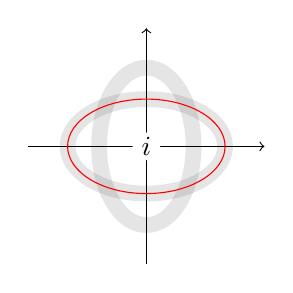
\begin{tikzpicture}[baseline = -2.8pt]
      \draw [->] (-1.5,0) -- (1.5,0);
      \draw [->] (0,-1.5) -- (0,1.5);
      \draw [line width = .2cm, opacity = .1] (0,0) ellipse (1 and .6);
      \draw [line width = .2cm, opacity = .1] (0,0) ellipse (.6 and 1);
      \node [circle, fill = white, inner sep = 0pt,
             minimum width = 1em, minimum height = 1em]
        at (0,0) {$i$};
      \draw [red] (0,0) ellipse (1 and .6);
    \end{tikzpicture}\enspace
    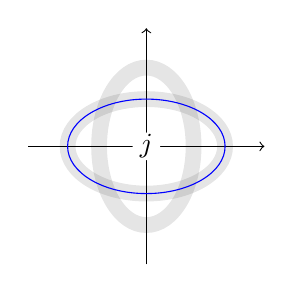
\begin{tikzpicture}[baseline = -2.8pt]
      \draw [->] (-1.5,0) -- (1.5,0);
      \draw [->] (0,-1.5) -- (0,1.5);
      \draw [line width = .2cm, opacity = .1] (0,0) ellipse (1 and .6);
      \draw [line width = .2cm, opacity = .1] (0,0) ellipse (.6 and 1);
      \node [circle, fill = white, inner sep = 0pt,
             minimum width = 1em, minimum height = 1em]
        at (0,0) {$j$};
      \draw [blue] (0,0) ellipse (1 and .6);
    \end{tikzpicture}
    \xlongrightarrow{\mathcal V_{i\to j}}
    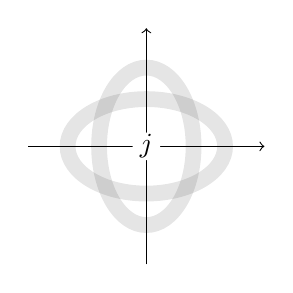
\begin{tikzpicture}[baseline = -2.8pt]
      \draw [->] (-1.5,0) -- (1.5,0);
      \draw [->] (0,-1.5) -- (0,1.5);
      \draw [line width = .2cm, opacity = .1] (0,0) ellipse (1 and .6);
      \draw [line width = .2cm, opacity = .1] (0,0) ellipse (.6 and 1);
      \node [circle, fill = white, inner sep = 0pt,
             minimum width = 1em, minimum height = 1em]
        at (0,0) {$j$};
    \end{tikzpicture}\enspace
    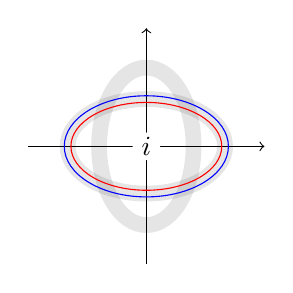
\begin{tikzpicture}[baseline = -2.8pt]
      \draw [->] (-1.5,0) -- (1.5,0);
      \draw [->] (0,-1.5) -- (0,1.5);
      \draw [line width = .2cm, opacity = .1] (0,0) ellipse (1 and .6);
      \draw [line width = .2cm, opacity = .1] (0,0) ellipse (.6 and 1);
      \node [circle, fill = white, inner sep = 0pt,
             minimum width = 1em, minimum height = 1em]
        at (0,0) {$i$};
      \draw [red] (0,0) ellipse ({1cm - 1.2pt} and {.6cm - 1.2pt});
      \draw [blue] (0,0) ellipse ({1cm + 1.2pt} and {.6cm + 1.2pt});
    \end{tikzpicture}\tag{Fig. 1}\label{hops_fig:1}\\
    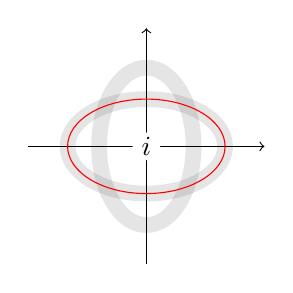
\begin{tikzpicture}[baseline = -2.8pt]
      \draw [->] (-1.5,0) -- (1.5,0);
      \draw [->] (0,-1.5) -- (0,1.5);
      \draw [line width = .2cm, opacity = .1] (0,0) ellipse (1 and .6);
      \draw [line width = .2cm, opacity = .1] (0,0) ellipse (.6 and 1);
      \node [circle, fill = white, inner sep = 0pt,
             minimum width = 1em, minimum height = 1em]
        at (0,0) {$i$};
      \draw [red] (0,0) ellipse (1 and .6);
    \end{tikzpicture}\enspace
    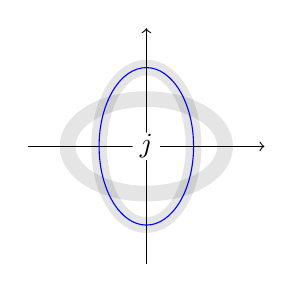
\begin{tikzpicture}[baseline = -2.8pt]
      \draw [->] (-1.5,0) -- (1.5,0);
      \draw [->] (0,-1.5) -- (0,1.5);
      \draw [line width = .2cm, opacity = .1] (0,0) ellipse (1 and .6);
      \draw [line width = .2cm, opacity = .1] (0,0) ellipse (.6 and 1);
      \node [circle, fill = white, inner sep = 0pt,
             minimum width = 1em, minimum height = 1em]
        at (0,0) {$j$};
      \draw [blue] (0,0) ellipse (.6 and 1);
    \end{tikzpicture}
    \xlongrightarrow{\mathcal V_{i\to j}}
    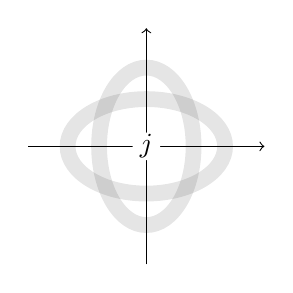
\begin{tikzpicture}[baseline = -2.8pt]
      \draw [->] (-1.5,0) -- (1.5,0);
      \draw [->] (0,-1.5) -- (0,1.5);
      \draw [line width = .2cm, opacity = .1] (0,0) ellipse (1 and .6);
      \draw [line width = .2cm, opacity = .1] (0,0) ellipse (.6 and 1);
      \node [circle, fill = white, inner sep = 0pt,
             minimum width = 1em, minimum height = 1em]
        at (0,0) {$j$};
    \end{tikzpicture}\enspace
    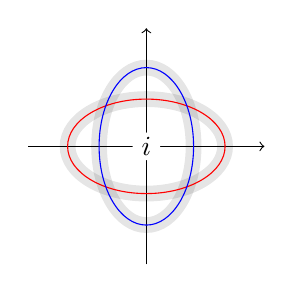
\begin{tikzpicture}[baseline = -2.8pt]
      \draw [->] (-1.5,0) -- (1.5,0);
      \draw [->] (0,-1.5) -- (0,1.5);
      \draw [line width = .2cm, opacity = .1] (0,0) ellipse (1 and .6);
      \draw [line width = .2cm, opacity = .1] (0,0) ellipse (.6 and 1);
      \node [circle, fill = white, inner sep = 0pt,
             minimum width = 1em, minimum height = 1em]
        at (0,0) {$i$};
      \draw [red] (0,0) ellipse (1 and .6);
      \draw [blue] (0,0) ellipse (.6 and 1);
    \end{tikzpicture}\tag{Fig. 2}\label{hops_fig:2}\\
    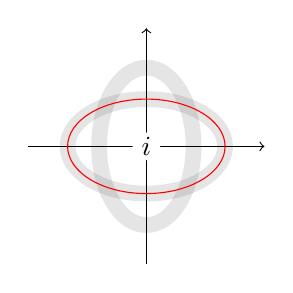
\begin{tikzpicture}[baseline = -2.8pt]
      \draw [->] (-1.5,0) -- (1.5,0);
      \draw [->] (0,-1.5) -- (0,1.5);
      \draw [line width = .2cm, opacity = .1] (0,0) ellipse (1 and .6);
      \draw [line width = .2cm, opacity = .1] (0,0) ellipse (.6 and 1);
      \node [circle, fill = white, inner sep = 0pt,
             minimum width = 1em, minimum height = 1em]
        at (0,0) {$i$};
      \draw [red] (0,0) ellipse (1 and .6);
    \end{tikzpicture}\enspace
    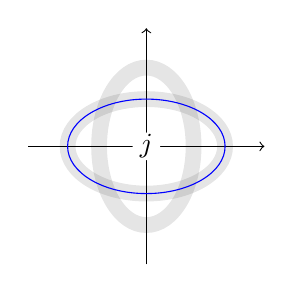
\begin{tikzpicture}[baseline = -2.8pt]
      \draw [->] (-1.5,0) -- (1.5,0);
      \draw [->] (0,-1.5) -- (0,1.5);
      \draw [line width = .2cm, opacity = .1] (0,0) ellipse (1 and .6);
      \draw [line width = .2cm, opacity = .1] (0,0) ellipse (.6 and 1);
      \node [circle, fill = white, inner sep = 0pt,
             minimum width = 1em, minimum height = 1em]
        at (0,0) {$j$};
      \draw [blue] (0,0) ellipse (1 and .6);
    \end{tikzpicture}
    \xlongrightarrow{\mathcal V_{j\to i}}
    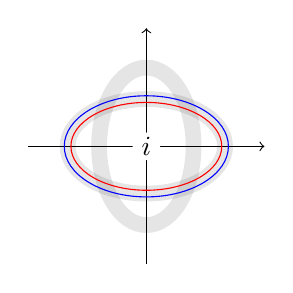
\begin{tikzpicture}[baseline = -2.8pt]
      \draw [->] (-1.5,0) -- (1.5,0);
      \draw [->] (0,-1.5) -- (0,1.5);
      \draw [line width = .2cm, opacity = .1] (0,0) ellipse (1 and .6);
      \draw [line width = .2cm, opacity = .1] (0,0) ellipse (.6 and 1);
      \node [circle, fill = white, inner sep = 0pt,
             minimum width = 1em, minimum height = 1em]
        at (0,0) {$i$};
      \draw [red] (0,0) ellipse ({1cm - 1.2pt} and {.6cm - 1.2pt});
      \draw [blue] (0,0) ellipse ({1cm + 1.2pt} and {.6cm + 1.2pt});
    \end{tikzpicture}\enspace
    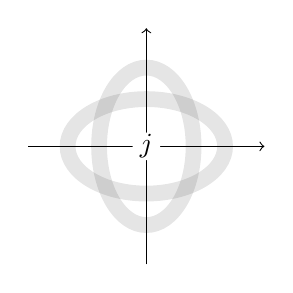
\begin{tikzpicture}[baseline = -2.8pt]
      \draw [->] (-1.5,0) -- (1.5,0);
      \draw [->] (0,-1.5) -- (0,1.5);
      \draw [line width = .2cm, opacity = .1] (0,0) ellipse (1 and .6);
      \draw [line width = .2cm, opacity = .1] (0,0) ellipse (.6 and 1);
      \node [circle, fill = white, inner sep = 0pt,
             minimum width = 1em, minimum height = 1em]
        at (0,0) {$j$};
    \end{tikzpicture}\tag{Fig. 3}\label{hops_fig:3}\\
    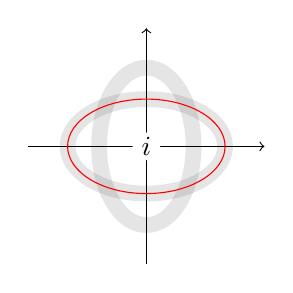
\begin{tikzpicture}[baseline = -2.8pt]
      \draw [->] (-1.5,0) -- (1.5,0);
      \draw [->] (0,-1.5) -- (0,1.5);
      \draw [line width = .2cm, opacity = .1] (0,0) ellipse (1 and .6);
      \draw [line width = .2cm, opacity = .1] (0,0) ellipse (.6 and 1);
      \node [circle, fill = white, inner sep = 0pt,
             minimum width = 1em, minimum height = 1em]
        at (0,0) {$i$};
      \draw [red] (0,0) ellipse (1 and .6);
    \end{tikzpicture}\enspace
    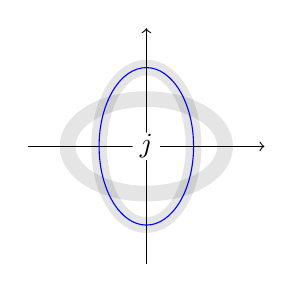
\begin{tikzpicture}[baseline = -2.8pt]
      \draw [->] (-1.5,0) -- (1.5,0);
      \draw [->] (0,-1.5) -- (0,1.5);
      \draw [line width = .2cm, opacity = .1] (0,0) ellipse (1 and .6);
      \draw [line width = .2cm, opacity = .1] (0,0) ellipse (.6 and 1);
      \node [circle, fill = white, inner sep = 0pt,
             minimum width = 1em, minimum height = 1em]
        at (0,0) {$j$};
      \draw [blue] (0,0) ellipse (.6 and 1);
    \end{tikzpicture}
    \xlongrightarrow{\mathcal V_{j\to i}}
    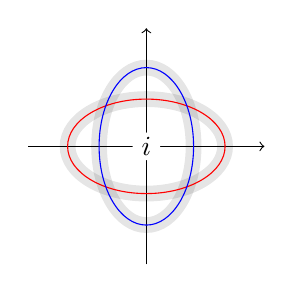
\begin{tikzpicture}[baseline = -2.8pt]
      \draw [->] (-1.5,0) -- (1.5,0);
      \draw [->] (0,-1.5) -- (0,1.5);
      \draw [line width = .2cm, opacity = .1] (0,0) ellipse (1 and .6);
      \draw [line width = .2cm, opacity = .1] (0,0) ellipse (.6 and 1);
      \node [circle, fill = white, inner sep = 0pt,
             minimum width = 1em, minimum height = 1em]
        at (0,0) {$i$};
      \draw [red] (0,0) ellipse (1 and .6);
      \draw [blue] (0,0) ellipse (.6 and 1);
    \end{tikzpicture}\enspace
    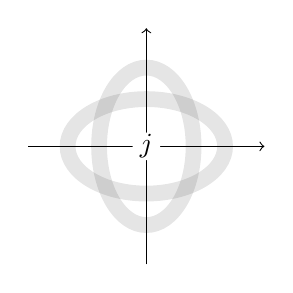
\begin{tikzpicture}[baseline = -2.8pt]
      \draw [->] (-1.5,0) -- (1.5,0);
      \draw [->] (0,-1.5) -- (0,1.5);
      \draw [line width = .2cm, opacity = .1] (0,0) ellipse (1 and .6);
      \draw [line width = .2cm, opacity = .1] (0,0) ellipse (.6 and 1);
      \node [circle, fill = white, inner sep = 0pt,
             minimum width = 1em, minimum height = 1em]
        at (0,0) {$j$};
    \end{tikzpicture}\tag{Fig. 4}\label{hops_fig:4}
  \end{gather}
  where different colors correspond to different spin directions, and the
  hop like
  \[
    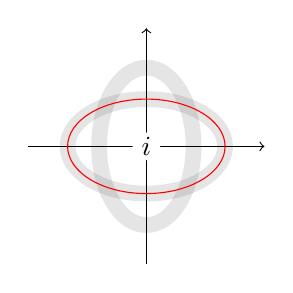
\begin{tikzpicture}[remember picture, baseline = -2.8pt]
      \coordinate (a) at (-1.5,1.5);
      \coordinate (c) at (-1.5,-1.5);
      \draw [->] (-1.5,0) -- (1.5,0);
      \draw [->] (0,-1.5) -- (0,1.5);
      \draw [line width = .2cm, opacity = .1] (0,0) ellipse (1 and .6);
      \draw [line width = .2cm, opacity = .1] (0,0) ellipse (.6 and 1);
      \node [circle, fill = white, inner sep = 0pt,
             minimum width = 1em, minimum height = 1em]
        at (0,0) {$i$};
      \draw [red] (0,0) ellipse (1 and .6);
    \end{tikzpicture}\enspace
    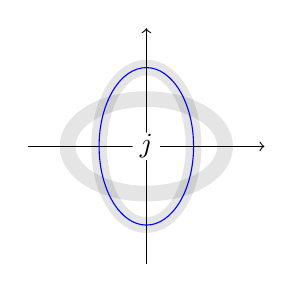
\begin{tikzpicture}[baseline = -2.8pt]
      \draw [->] (-1.5,0) -- (1.5,0);
      \draw [->] (0,-1.5) -- (0,1.5);
      \draw [line width = .2cm, opacity = .1] (0,0) ellipse (1 and .6);
      \draw [line width = .2cm, opacity = .1] (0,0) ellipse (.6 and 1);
      \node [circle, fill = white, inner sep = 0pt,
             minimum width = 1em, minimum height = 1em]
        at (0,0) {$j$};
      \draw [blue] (0,0) ellipse (.6 and 1);
    \end{tikzpicture}
    \xlongrightarrow{\mathcal V_{i\to j}}
    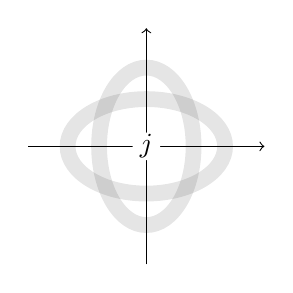
\begin{tikzpicture}[baseline = -2.8pt]
      \draw [->] (-1.5,0) -- (1.5,0);
      \draw [->] (0,-1.5) -- (0,1.5);
      \draw [line width = .2cm, opacity = .1] (0,0) ellipse (1 and .6);
      \draw [line width = .2cm, opacity = .1] (0,0) ellipse (.6 and 1);
      \node [circle, fill = white, inner sep = 0pt,
             minimum width = 1em, minimum height = 1em]
        at (0,0) {$j$};
    \end{tikzpicture}\enspace
    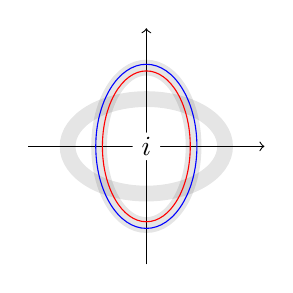
\begin{tikzpicture}[remember picture, baseline = -2.8pt]
      \draw [->] (-1.5,0) -- (1.5,0);
      \draw [->] (0,-1.5) -- (0,1.5);
      \draw [line width = .2cm, opacity = .1] (0,0) ellipse (1 and .6);
      \draw [line width = .2cm, opacity = .1] (0,0) ellipse (.6 and 1);
      \node [circle, fill = white, inner sep = 0pt,
             minimum width = 1em, minimum height = 1em]
        at (0,0) {$i$};
      \draw [red] (0,0) ellipse ({.6cm - 1.2pt} and {1cm - 1.2pt});
      \draw [blue] (0,0) ellipse ({.6cm + 1.2pt} and {1cm + 1.2pt});
      \coordinate (b) at (1.5,1.5);
      \coordinate (d) at (1.5,-1.5);
    \end{tikzpicture}
    \begin{tikzpicture}[remember picture, overlay]
      \draw [thin, red] (a) -- (d);
      \draw [thin, red] (b) -- (c);
    \end{tikzpicture}
  \]
  is not allowed.
  In the large-$U$ limit ($t \ll U$, $U'$, $J_H$), the atomic term
  determines the atomic eigenstates and energies. For a fixed site $i$, we can
  obtain its energy by substituting 2 different situations
  into $\mathcal H^\text{loc}$.
  \begin{enumext}
    \item \textbf{Both electrons in the same orbital $m$.}
    Due to Pauli exclusion, the spins must be opposite: One $\uparrow$
    and one $\downarrow$. The four terms are
    \begin{enumext}
      \item $n_{\uparrow,m} n_{\downarrow,m}$ satisfies the same orbital $m$ and
      different spin directions. So, $n_{\uparrow,m} n_{\downarrow,m} = 1$.
      \item Expanding the second term first
      \[
        (n_{i,\uparrow,1} + n_{i,\downarrow,1})
        (n_{i,\uparrow,2} + n_{i,\downarrow,2})
      = n_{i,\uparrow,1}    n_{i,\uparrow,2}
      + n_{i,\downarrow,1}  n_{i,\uparrow,2}
      + n_{i,\uparrow,1}    n_{i,\downarrow,2}
      + n_{i,\downarrow,1}  n_{i,\downarrow,2}.
      \]
      The expanded 4 terms are in different orbitals $1$ and $2$,
      so $(n_{i,\uparrow,1} + n_{i,\downarrow,1})
          (n_{i,\uparrow,2} + n_{i,\downarrow,2}) = 0$.
      \item Obviously, $\vec S_1 \cdot \vec S_2 = 0$ since both electrons occupy
      the same orbital and one of $\vec S$ is zero.
      \item For the last term, calculate the denominator for the
      second-order perturbation,
      \[
        \Delta E = E_\text{ext} - E_\text{int}.
      \]
      \begin{enumext}[label = \arabic*.]
        \item Initial state: There is one electron in the two neighbor site,
        then $E_\text{int} = (-\mu) + (-\mu) = -2\mu$.
        \item Excited state: There are two electrons in one site, leaving
        another empty. Then a Coulomb potential is applied,
        $E_\text{ext} = \tilde U + (-\mu) + (-\mu) = U - 2\mu$.
      \end{enumext}
      This chemical potential term cancels in the energy denominator and
      therefore does not contribute.
    \end{enumext}
    In summary, the energy in this case is
    \[
      E_\text{same} = U \cdot 1 + (U' - J_H/2) \cdot 0 - 2J_H \cdot 0 - 0 = U.
    \]
    \item \textbf{Electrons in different orbitals}
    Let the electron in orbital 1 has spin $\sigma_1$, the electron in orbital
    2 has spin $\sigma_2$. The four terms are
    \begin{enumext}
      \item $n_{\uparrow,m} n_{\downarrow,m}$ is obviously zero, since they are
      at the same orbital.
      \item In each bracket of $(n_{i,\uparrow,1} + n_{i,\downarrow,1})
        (n_{i,\uparrow,2} + n_{i,\downarrow,2})$, only one term can be $1$
      and another one should be $0$. So, this term gives a value
      of $1 \times 1 = 1$.
      \item The Hund term couples the spins of the two orbitals
      \[
        \vec S_1 \cdot \vec S_2
      = \frac12\ab[(\vec S_1 + \vec S_2)^2 - \vec S_1^2 - \vec S_2^2]
      = \frac12\ab(|\vec S|^2 - \frac34 - \frac34)
      = \frac12\ab(|\vec S|^2 - \frac32),
      \]
      where each $\vec S_m$ corresponds to spin-$\frac12$ of the electron in
      orbital $m$, so $\vec S_m^2 = \frac34$.
      The total spin $\vec S = \vec S_1 + \vec S_2$ has the
      \begin{enumext}
        \item Triplet: $|\vec S| = 1$,
        then $\vec S^2 = |\vec S|(|\vec S| + 1) = 2$,
        $\vec S_1 \cdot \vec S_2 = \frac12\ab(2 - \frac32) = \frac14$.
        \item Singlet: $|\vec S| = 0$, then $\vec S^2 = 0$,
        $\vec S_1 \cdot \vec S_2 = \frac12\ab(0 - \frac32) = -\frac34$.
      \end{enumext}
      \item The same as the case (a). This term vanishes.
    \end{enumext}
    In summary, the energy in this case is
    \[
      E_\text{diff} =
      \begin{cases*}
        (U' - \frac{J_H}2) - 2J_H \times \frac14 = U' - J_H,       & Triplet,\\
        (U' - \frac{J_H}2) - 2J_H \times \ab(-\frac34) = U' + J_H, & Singlet.
      \end{cases*}
    \]
  \end{enumext}
  Now, move on to the problems.
  \begin{enumext}[label = \Roman*.]
    \item Consider an electron hopping from site $i$ to $j$ (or inverse), one
    can have site $j$ doubly occupied and leave site $i$ empty (or inverse).
    The double occupancy have the energies
    \begin{enumext*}[label = (\alph*), columns = 61]
      \item(13) Same orbital: $U$.
      \item(24) Different orbitals, triplet: $U' - J_H$.
      \item(24) Different orbitals, singlet: $U' + J_H$.
    \end{enumext*}
    which has been referred to in the preparation work: (a) - iv.
    \begin{enumext}
      \item Same orbital: $m_i = m_j = m$, with the energy denominator $U$.\\
      When an electron from orbital $m$ on site $i$ hops to the same orbital of
      the site $j$, this gives double occupancy in the same orbital $m$ on
      site $j$; Also for the inverse. So, the perturbation can be written as
      \[
        \mathcal V = \mathcal V_{i\to j} + \mathcal V_{j\to i}, \quad
        \mathcal V_{i\to j}
      = t_{ij} \sum_\sigma c_{j,\sigma,m}^\dagger c_{i,\sigma,m}, \quad
        \mathcal V_{j\to i}
      = t_{ij} \sum_\sigma c_{i,\sigma,m}^\dagger c_{j,\sigma,m}.
      \]
      Due to the symmetry, the small hopping coefficients $t_{ji}$ are the same
      in the two hopping directions. Since the orbital is fixed, due to Pauli
      exclusion, the initial state of an arbitrary single bond $\braket<ij>$ can
      be \emph{only} the spin-singlet state
      \[
        \ket|S_{ij}> = \frac1{\sqrt2}
          (\ket|\uparrow_i\downarrow_j> - \ket|\downarrow_i\uparrow_j>)
      = \frac1{\sqrt2} \ab(
          c_{i,\uparrow}^\dagger c_{j,\downarrow}^\dagger
        - c_{i,\downarrow}^\dagger c_{j,\uparrow}^\dagger) \ket|0>.
      \]
      Applying $\mathcal V$ on it to obtain the numerator of the
      perturbed energy. In this case, consider each electron is moving in the
      same arbitrary orbit, then the orbital label can be omitted.
      \begin{enumext}[label = \arabic*.]
        \item Hopping from $i$ to $j$.
        \[
          \mathcal V_{i\to j} \ket|S_{ij}>
        = \frac{t_{ij}}{\sqrt2} \sum_\sigma
          c_{j,\sigma}^\dagger c_{i,\sigma} \ab(
          c_{i,\uparrow}^\dagger c_{j,\downarrow}^\dagger
        - c_{i,\downarrow}^\dagger c_{j,\uparrow}^\dagger) \ket|0>.
        \]
        The kernel of $\mathcal V_{i\to j} \ket|S_{ij}>$ is
        \begin{align*}
          \sum_\sigma \ab[c_{j,\sigma}^\dagger c_{i,\sigma}
          c_{i,\uparrow}^\dagger c_{j,\downarrow}^\dagger
        - c_{j,\sigma}^\dagger c_{i,\sigma}
          c_{i,\downarrow}^\dagger c_{j,\uparrow}^\dagger]
        = & \sum_\sigma \ab[c_{j,\sigma}^\dagger (\delta_{\sigma,\uparrow} -
          c_{i,\uparrow}^\dagger c_{i,\sigma})   c_{j,\downarrow}^\dagger
        - c_{j,\sigma}^\dagger (\delta_{\sigma,\downarrow} -
          c_{i,\downarrow}^\dagger c_{i,\sigma}) c_{j,\uparrow}^\dagger]\\
        = & \sum_\sigma \ab[\delta_{\sigma,\uparrow}
            c_{j,\sigma}^\dagger c_{j,\downarrow}^\dagger
        - \delta_{\sigma,\downarrow}
          c_{j,\sigma}^\dagger c_{j,\uparrow}^\dagger]
        = 2c_{j,\uparrow}^\dagger c_{j,\downarrow}^\dagger,
        \end{align*}
        where we used the anticommutative relation of Fermions
        \[
          \{c_{i,\sigma}^\dagger, c_{j,\sigma'}^\dagger\} = 0, \quad
          \{c_{i,\sigma}, c_{j,\sigma'}^\dagger\}
        = \delta_{ij}\delta_{\sigma\sigma'}.
        \]
        Hence, we can obtain
        \[
          \mathcal V_{i\to j} \ket|S_{ij}>
        = \sqrt2 t_{ij} \ket|0_i;\uparrow_j,\downarrow_j>
        = \sqrt2 t_{ij} \ket|\text{Doublon at $j$, empty at $i$}>.
        \]
        According to the perturbation theory, in the numerator of the perturbed
        energy
        \[
          \Delta E_a^{(2)}
        = -\sum_v \frac{|\braket<v|\mathcal V|a>|^2}{E_v - E_a}
        \]
        contains all possible intermediate states that are not in the low-energy
        manifold. So, this case contributes to the numerator
        \[
          |\braket<\text{Doublon at $j$, empty at $i$}|
          \mathemph[S_j]{\mathcal V_{i\to j}}|\mathemph[S_j]{S_{ij}}>|^2
        = 2t_{ij}^2.
        \]
        The colored block indicates the action target of $\mathcal V_{i\to j}$.
        \item Symmetrically, this case contributes
        \[
          |\braket<\mathemph[S_j]{\text{Doublon at $i$, empty at $j$}}|
          \mathemph[S_j]{\mathcal V_{j\to i}}|S_{ij}>|^2
        = 2t_{ij}^2,
        \]
        since they cause a symmetric result (See~\ref{hops_fig:1}
        and~\ref{hops_fig:3}).
      \end{enumext}
      In summary, By substituting the contributions into the perturbation
      theory, the total energy correction of the case
      \underline{same orbital \& singlet} is
      \begin{equation}
        \Delta E_\text{same, singlet}
        = -\ab(\frac{2t_{ij}^2}{U} + \frac{2t_{ij}^2}{U})
        = -\frac{4t_{ij}^2}{U}.
        \label{energy:same_orbital}
      \end{equation}
      To obtain the perturbed Hamiltonian for this part, define the operators
      for filtering the states with the case of the same orbital
      \[
        P_{ij}^\text{same} =
        \begin{rcases}
        \begin{cases}
          1, & m_i = m_j,\\
          0, & \text{otherwise}
        \end{cases}
        \end{rcases} = \frac12 + 2\tau_i^z \tau_j^z, \quad
        P_{ij}^\text{diff} = 1 - P_{ij}^\text{same}
      = \frac12 - 2\tau_i^z \tau_j^z.
      \]
      where $\tau^z = \pm\frac12$ is the orbital pseudospin, and operators for
      filtering the singlet and triplet states
      \[
        P_{ij}^S = \frac14 - \vec S_i \cdot \vec S_j, \quad
        P_{ij}^T = \frac34 + \vec S_i \cdot \vec S_j
      \]
      from the properties of the singlet $\vec S_i \cdot \vec S_j = -\frac34$
      and the triplet $\vec S_i \cdot \vec S_j = \frac14$. Now, we can write the
      Hamiltonian for this part
      \[
        \mathcal H_\text{same}^{ij}
      = -\frac{4t_{ij}^2}{U} P_{ij}^\text{same} P_{ij}^S.
      \]
      \item Different orbitals: $m_i \neq m_j$.\\
      Consider an arbitrary initial state
      \begin{enumext}[columns = 2, label = \arabic*.]
        \item Site $i$: Orbital $m = 1$, spin $\sigma_1$,
        \item Site $j$: Orbital $m = 2$, spin $\sigma_2$,
      \end{enumext}
      which can be expressed as
      \[
        \ket|S_{ij}>
      = c_{i,\sigma_1,1}^\dagger c_{j,\sigma_2,2}^\dagger \ket|0>,
      \]
      and there are two allowed processes for it
      \begin{enumext}[label = \arabic*.]
        \item Electron hops from $i$ (orbital 1) to $j$ (orbital 1).
        \item Electron hops from $j$ (orbital 2) to $i$ (orbital 2).
      \end{enumext}
      They will also cause a symmetric result (see figures~\ref{hops_fig:2}
      and~\ref{hops_fig:4}) like in part (i).
      So, analyze one process in parallel spins case and antiparallel
      spins case is enough.
      \begin{enumext}[label = \arabic*.]
        \item Parallel Spins Case: Take the spin
        directions $\sigma_i = \sigma_j = \uparrow$.\\
        The initial state now becomes
        \[
          \ket|\psi_\text{para}> = c_{i,\uparrow,1}^\dagger
            c_{j, \uparrow, 2}^\dagger \ket|0>.
        \]
        In the first process
        \begin{align*}
          \mathcal V_{i\to j}^{(1)} \ket|\psi_\text{para}> &
        = t_{ij} \sum_\sigma c_{j,\sigma,1}^\dagger c_{i,\sigma,1}
          c_{i,\uparrow,1}^\dagger c_{j,\uparrow,2}^\dagger \ket|0>
        = t_{ij} \sum_\sigma c_{j,\sigma,1}^\dagger
          (\delta_{\sigma,\uparrow} - c_{i,\uparrow,1}^\dagger c_{i,\sigma,1})
          c_{j,\uparrow,2}^\dagger \ket|0>\\
      & = t_{ij} c_{j,\uparrow,1}^\dagger c_{j,\uparrow,2}^\dagger \ket|0>
        = t_{ij} \ket|0_i;\uparrow_j\uparrow_j>.
        \end{align*}
        This is a state with two electrons at $j$: One in orbital 1 parallels
        to another one in orbital 2, corresponding to a triplet configuration,
        and the second process will give a similar result.
        They will contribute to the perturbed energy
        \begin{equation}
          \Delta E_\text{diff, para}
          = -2 \times \frac{|\braket<\uparrow_j\uparrow_j;0_i|t_{ij}|
          0_i;\uparrow_j\uparrow_j>|^2} {E_\text{diff,triplet}}
          = -\frac{2t_{ij}^2}{U' - J_H}.
          \label{energy:diff_orbital_para}
        \end{equation}
        \item Antiparallel Spins Case: Take the spin
        directions $\sigma_i = \uparrow$, $\sigma_j = \downarrow$.\\
        The initial state now becomes
        \[
          \ket|\psi_\text{anti}> = c_{i,\uparrow,1}^\dagger
            c_{j, \downarrow, 2}^\dagger \ket|0>.
        \]
        In the first process
        \begin{align*}
          \mathcal V_{i\to j}^{(1)} \ket|\psi_\text{anti}> &
        = t_{ij} \sum_\sigma c_{j,\sigma,1}^\dagger c_{i,\sigma,1}
          c_{i,\uparrow,1}^\dagger c_{j,\downarrow,2}^\dagger \ket|0>
        = t_{ij} \sum_\sigma c_{j,\sigma,1}^\dagger
          (\delta_{\sigma,\uparrow} - c_{i,\uparrow,1}^\dagger c_{i,\sigma,1})
          c_{j,\downarrow,2}^\dagger \ket|0>\\
      & = t_{ij} c_{j,\uparrow,1}^\dagger c_{j,\downarrow,2}^\dagger \ket|0>
        = t_{ij} \ket|0_i;\uparrow_j\downarrow_j>.
        \end{align*}
        This is a 50-50 mixture of triplet and singlet
        \[
          \ket|\uparrow\downarrow>
        = \frac1{\sqrt2}\ab[\frac1{\sqrt2}
            (\ket|\uparrow\downarrow> + \ket|\downarrow\uparrow>)
          + \frac1{\sqrt2}
            (\ket|\uparrow\downarrow> - \ket|\downarrow\uparrow>)]
        = \frac1{\sqrt2}(\ket|T> + \ket|S>),
        \]
        and the two parts will contribute
        \begin{equation}
          \Delta E_\text{diff, anti} = -\ab(
          \frac{|\braket<T|t_{ij}|T>|^2}{U' - J_H}
        + \frac{|\braket<S|t_{ij}|S>|^2}{U' + J_H})
        = -\frac{t_{ij}^2}{U' - J_H} - \frac{t_{ij}^2}{U' + J_H}
          \label{energy:diff_orbital_anti}
          \end{equation}
        to the correction.
      \end{enumext}
      In summary, to obtain the perturbed Hamiltonian for the case
      \underline{different orbitals}, using the defined projectors and
      combining the two cases with the coefficients
      \[
        \mathcal H_\text{diff}^{ij}
      = -\frac{2t_{ij}^2}{U' - J_H} P_{ij}^\text{diff} P_{ij}^T
        -\frac{2t_{ij}^2}{U' + J_H} P_{ij}^\text{diff} P_{ij}^S.
      \]
      to make this part Hamiltonian satisfy
      at $P_{ij}^\text{diff} = 1$
      \[
        \mathcal H_\text{diff}^{ij} =
        \begin{cases}
          -\frac{2t^2}{U' - J_H}, & P^T = 1,\ P^S = 0,\\
          -\frac{t^2}{U' - J_H} - \frac{t^2}{U' + J_H}, & P^T = P^S = \frac12.
        \end{cases}
      \]
    \end{enumext}
    By summing, we can obtain the compact form of the second-order perturbed
    Hamiltonian
    \[
      \mathcal H_{ij}^{(2)} = -\frac{4t_{ij}^2}{U} P_{ij}^\text{same} P_{ij}^S
    - \frac{2t_{ij}^2}{U' - J_H} P_{ij}^\text{diff} P_{ij}^T
    - \frac{2t_{ij}^2}{U' + J_H} P_{ij}^\text{diff} P_{ij}^S.
    \]
    Substituting the projection operators, we obtained the perturbed
    Hamiltonian in Kugel-Khomskii operator form
    \begin{multline}
      \mathcal H_{ij}^{(2)}
    = -\frac{t_{ij}^2}2 \ab(\frac 1U + \frac{2U' + J_H}{U'^2 - J_H^2})
    + 2t_{ij}^2\ab(\frac1U - \frac{J_H}{U'^2 - J_H^2}) \vec S_i \cdot \vec S_j\\
    + 2t_{ij}^2\ab(-\frac1U + \frac{2U' + J_H}{U'^2 - J_H^2}) \tau_i^z \tau_j^z
    + 8t_{ij}^2\ab(\frac1U + \frac{J_H}{U'^2 - J_H^2})
      (\vec S_i \cdot \vec S_j) (\tau_i^z \tau_j^z).
    \label{eq:2nd_ptb_h}
    \end{multline}
    \item One can construct a N\'eel-type product state, but for realistic
    Hund's coupling $J_H$ the ground state is typically a ferromagnetic spin
    order with staggered orbital order due to Hund-enhanced ferromagnetic
    exchange on inter-orbital bonds.
    \begin{proof}
      Evaluate the energy for the semi-classical ground energy of a
      bond $\braket<ij>$
      \[
        E_{ij}^\text{class}
      = \braket<\Psi_\text{class}|\mathcal H_{ij}^{(2)}|\Psi_\text{class}>,
      \]
      where the state can be written as
      \[
        \ket|\Psi_\text{class}> = \bigotimes_i
        \ket|\hat n_i>_\text{spin} \otimes \ket|\tau_i^z>_\text{orbital}.
      \]
      in which $\hat n_i$ denotes the spin direction, and $\tau_i^z$ denotes the
      orbital occupation: $\tau_i^z = \pm\frac12$ for either orbital 1 or
      orbital 2. For a product state with fixed spin directions and
      orbital pseudospins
      \[
        \braket<\vec S_i \cdot \vec S_j> = S^2 \cos\theta_{ij}
      = \frac14 \cos\theta_{ij}, \quad
        \braket<\tau_i^z \tau_j^z> = \tau_i \tau_j, \quad \tau_i^z = \pm\frac12,
      \]
      where $\theta_{ij}$ denotes the angle between spin directions at site $i$
      and $j$. Thus, the expectation values of the projectors can be
      expressed as
      \[
        \braket<P_{ij}^S> = \frac14(1 - \cos\theta_{ij}), \quad
        \braket<P_{ij}^T> = \frac14(3 + \cos\theta_{ij}), \quad
        \braket<P_{ij}^\text{same}> = \frac12 + 2\tau_i\tau_j,\quad
        \braket<P_{ij}^\text{diff}> = \frac12 - 2\tau_i\tau_j.
      \]
      Now, the uncertain variables are $\theta_{ij}$ and $\tau_i\tau_j$.
      For simplicity, define the three exchange scales
      \[
        J_1 \equiv \frac{4t_{ij}^2}{U}, \quad
        J_- \equiv \frac{2t_{ij}^2}{U' - J_H}, \quad
        J_+ \equiv \frac{2t_{ij}^2}{U' + J_H}.
      \]
      Then, we can analyze bond energies in two different cases.
      \begin{enumext}[label = (\alph*)]
        \item Same orbital bond: $\tau_i \tau_j = +\frac14$. The projectors
        now become
        \[
          \braket<P_{ij}^\text{same}> = \frac12 + 2 \times \frac14 = 1, \quad
          \braket<P_{ij}^\text{diff}> = \frac12 - 2 \times \frac14 = 0.
        \]
        Then, the energy
        \[
          E_{ij}^\text{same} = -\frac{4t_{ij}^2}{U}
          \braket<P_{ij}^\text{same}> \braket<P_{ij}^S>
        = -\frac{t_{ij}^2}{U} (1 - \cos\theta_{ij})
        = -\frac{J_1}{4} (1 - \cos\theta_{ij}).
        \]
        We can obtain the minimum (at $\theta_{ij} = \pi$) and
        the maximum (at $\theta_{ij} = 0$), between which the lattice will
        behave like an antiferromagnetic, driven by Hund's exclusion
        \begin{equation}
          E_{\min}^\text{afm} = -\frac{J_1}{2}, \quad
          E_{\max}^\text{afm} = 0. \tag*{
          \textuparrow \textdownarrow \textuparrow \textdownarrow
          \textuparrow \textdownarrow \textuparrow \textdownarrow
          \textuparrow \textdownarrow \textuparrow \textdownarrow}
        \end{equation}
        \item Different orbital bond: $\tau_i \tau_j = -\frac14$. The
        projectors
        \[
          \braket<P_{ij}^\text{same}> = \frac12 - 2 \times \frac14 = 0, \quad
          \braket<P_{ij}^\text{diff}> = \frac12 + 2 \times \frac14 = 1.
        \]
        Then, the energy
        \begin{multline*}
          E_{ij}^\text{diff} = -\frac{2t_{ij}^2}{U' - J_H}
          \braket<P_{ij}^\text{diff}> \braket<P_{ij}^T>
          - \frac{2t_{ij}^2}{U' + J_H}
          \braket<P_{ij}^\text{diff}> \braket<P_{ij}^S>\\
        = - \frac{t_{ij}^2}{2}\ab[
              \frac{3 + \cos\theta_{ij}}{U' - J_H}
            + \frac{1 - \cos\theta_{ij}}{U' + J_H}]
        = -\frac{3J_- + J_+}{4} - \frac{J_- - J_+}{4} \cos\theta_{ij}.
        \end{multline*}
        Since $U' - J_H < U' + J_H$, so $J_- > J_+$, the coefficient
        of $-\cos\theta_{ij}$ is positive. Then, we can obtain the minimum
        (at $\theta_{ij} = 0$) and the maximum (at $\theta_{ij} = \pi$),
        between which the lattice will behave like ferromagnetic
        \begin{equation}
          E_{\min}^\text{fm} = -J_-, \quad
          E_{\max}^\text{fm} = -\frac12(J_- + J_+). \tag*{
          \textuparrow \textuparrow \textuparrow \textuparrow
          \textuparrow \textuparrow \textuparrow \textuparrow
          \textuparrow \textuparrow \textuparrow \textuparrow}
        \end{equation}
      \end{enumext}
      To judge which case has lower energy, just compare their minimal energies
      \[
        E_{\min}^\text{afm} = -\frac{J_1}{2} = -\frac{2t_{ij}^2}{U},\quad
        E_{\min}^\text{fm} = -J_- = -\frac{2t_{ij}^2}{U' - J_H},
      \]
      the lower one will win. Due to the rotational invariance in
      orbital space, $U' = U - 2J_H$, even without this relation, since the
      positive Hund's coupling, the ferromagnetic state has the lowest energy,
      which will be denoted as the ground state.

      Hence, a N\'eel-type product state can be constructed, but it is not the
      ground state for physically realistic parameters with nonzero Hund's
      coupling. Except \emph{in the absence of Hund's coupling ($J_H = 0$), the
      two energies become equal, and the N\'eel state would be both the ground
      state and also degenerate with the other state.}
      \hfill \ensuremath \square
    \end{proof}
    \item \begin{enumext}[label = (\alph*)]
      \item The retarded Green's function for orbital $m$, spin $\sigma$ on site
      $i$ is
      \[
        G_{m,\sigma}^i(\omega)
      = \ab*<\braket<c_{i,m,\sigma};c_{i,m,\sigma}^\dagger>>_\omega.
      \]
      In the atomic limit ($U \gg t$), one can compute the Green's function
      using Lehmann representation
      \[
        G_{m,\sigma}^i(\omega)
      = \sum_n \frac{|\braket<n|c_{i,m,\sigma}^\dagger|i>|^2}
          {\omega - (E_n - E_0) + \iu 0^+}
      + \sum_n \frac{|\braket<n|c_{i,m,\sigma}|i>|^2}
          {\omega + (E_n - E_0) + \iu 0^+},
      \]
      where $\ket|i> = c_{i,m_0,\sigma_0}^\dagger \ket|0>$ is the initial state
      for site $i$: $m_0$ can be taken as $1$ or $2$, and $\sigma_0$ can be
      taken as $\uparrow$ or $\downarrow$.
      Consider applying an annihilation or a creation operator for removal or
      addition to a site, due to the difference between $m$
      and $m_0$, $\sigma$ and $\sigma_0$, it can be divided into 4 cases
      \begin{enumext}[label = \roman*.]
        \item Same orbital, same spin ($m = m_0$, $\sigma = \sigma_0$).
        \begin{enumext}[label = \arabic*.]
          \item Removal:
          $c_{i,m_0,\sigma_0} c_{i,m_0,\sigma_0}^\dagger\ket|0> = \ket|0>$.
          \item Addition: Blocked by the Pauli exclusion principle, no
          addition pole.
        \end{enumext}
        The matrix element is $1$, the pole is $\omega = 0$. The Green's
        function is
        \[
          G^\text{same, same} = \frac1{\omega + \iu0^+}.
        \]
        \item Same orbital, different spin ($m = m_0$, $\sigma = -\sigma_0$).
        \begin{enumext}[label = \arabic*.]
          \item Removal:
          $c_{i,m_0,-\sigma_0} c_{i,m_0,\sigma_0}^\dagger\ket|0> = 0$ due to
          there is no spin $-\sigma_0$ at $m_0$ orbital for removal.
          \item Addition:
          $c_{i,m_0,-\sigma_0}^\dagger c_{i,m_0,\sigma_0}^\dagger\ket|0>
        = \ket|m_0,\sigma_0;m_0,-\sigma_0>$.
        \end{enumext}
        The matrix element is $1$, the pole is $\omega = U$. The Green's
        function is
        \[
          G^\text{same, diff} = \frac1{\omega - U + \iu0^+}.
        \]
        \item Different orbital, same spin ($m \neq m_0$, $\sigma = \sigma_0$).
        \begin{enumext}[label = \arabic*.]
          \item Removal:
          $c_{i,m,\sigma_0} c_{i,m_0,\sigma_0}^\dagger\ket|0> = 0$ due to there
          is no spin at $m$ orbital for removal.
          \item Addition:
          $c_{i,m,\sigma_0}^\dagger c_{i,m_0,\sigma_0}^\dagger\ket|0>
        = \ket|m_0,\sigma_0;m,\sigma_0>$, triplet.
        \end{enumext}
        The matrix element is $1$, the pole is $\omega = U' - J_H$. The Green's
        function is
        \[
          G^\text{diff, same} = \frac1{\omega - (U' - J_H)+ \iu0^+}.
        \]
        \item Different orbital, different spin
        ($m \neq m_0$, $\sigma = -\sigma_0$).
        \begin{enumext}[label = \arabic*.]
          \item Removal:
          $c_{i,m,-\sigma_0} c_{i,m_0,\sigma_0}^\dagger\ket|0> = 0$ due to there
          no spin at $m$ orbital for removal.
          \item Addition:
          $c_{i,m,-\sigma_0}^\dagger c_{i,m_0,\sigma_0}^\dagger\ket|0>
          = \ket|m_0,\sigma_0;m,-\sigma_0> = \frac1{\sqrt2}(\ket|T> + \ket|S>)$,
          50-50 mixture of triplet and singlet.
        \end{enumext}
        The matrix element for both triplet and singlet is $1/2$, the poles are
        $\omega = U' - J_H$ and $\omega = U' + J_H$. The Green's function is
        \[
          G^\text{diff,diff}
        = \frac12 \frac1{\omega - (U' - J_H) + \iu0^+}
        + \frac12 \frac1{\omega - (U' + J_H) + \iu0^+}.
        \]
      \end{enumext}
      \item Starting from the effective Hamiltonian in~\eqref{eq:2nd_ptb_h}, its
      expectation can be written as
      \[
        \braket<\mathcal H_{ij}^{(2)}>
      = J_s m^2 + J_\tau p^2 + J_{S_\tau} m^2p^2 + \text{Constant},
      \]
      where
      \[\begin{array}{*3{r@{~}c@{~}l}}
          J_S        & = & 2t_{ij}^2
                           \ab(\frac1U - \frac{J_H}{U'^2 - J_H^2}),       &
          J_\tau     & = & 2t_{ij}^2
                           \ab(-\frac1U + \frac{2U' + J_H}{U'^2 - J_H^2}),&
          J_{S_\tau} & = & 8t_{ij}^2
                           \ab(\frac1U + \frac{J_H}{U'^2 - J_H^2}),       \\
                 m^2 & = & \braket<\vec S_i \cdot \vec S_j>,              &
                 p^2 & = & \braket<\tau_i^z \tau_j^z>,                    &
     \text{Constant} & = &-\frac{t_{ij}^2}2
                           \ab(\frac 1U + \frac{2U' + J_H}{U'^2 - J_H^2}).
        \end{array}
      \]
      Summing over bonds gives the mean energy per site
      \[
        U_\text{Mean Field} = \frac{z}{2}
          (J_s m^2 + J_\tau p^2 + J_{S_\tau} m^2p^2),
      \]
      where $z$ is the coordination number, and a factor $\frac12$ is
      applied to avoid doubling when summing over $\braket<ij>$. Then, we can
      obtain the mean-field free energy per site by definition
      \[
        F_\text{Mean field} = U_\text{Mean Field} - Ts(m,p)
      = \frac z2 (J_s m^2 + J_\tau p^2 + J_{S_\tau} m^2p^2) - T[s(m) + s(p)].
      \]
      Then calculate the entropy. Denote $P_+$, $P_-$ the probability
      of $S^z = +\frac12$ and $S^z = -\frac12$ respectively. Then, the
      expectation of the magnetization is
      \[
        m = \braket<S^z> = \ab(\frac12)P_+ + \ab(-\frac12)P_-.
      \]
      Due to the normalization $P_+ + P_- = 1$, we can obtain
      \[
        P_+ = \frac12 + m, \quad P_- = \frac12 - m.
      \]
      Then, substitute them into the definition of the entropy
      \begin{align*}
        s_S(m) & = -\sum_i P_i \ln P_i
      = -[P_+\ln P_+ + P_-\ln P_-]\\
    & = -\ab[\ab(\frac12 + m) \ln\ab(\frac12 + m)
        + \ab(\frac12 - m) \ln\ab(\frac12 - m)].
      \end{align*}
      which satisfies $s_S(\pm\frac12) = 0$ for fully polarized states.
      For minimization, calculating the derivative of the entropy
      for magnetization, and similarly for polarization
      \[
        \pdv{s_S}m = -\ln\ab(\frac{1 + 2m}{1 - 2m}) = -2\tanh^{-1}(2m), \quad
        \pdv{s_S}p = -\ln\ab(\frac{1 + 2p}{1 - 2p}) = -2\tanh^{-1}(2p).
      \]
      Then, minimize the free energy with respect to $m$ and $p$: Let
      $\pdv{F_\text{Mean field}}/m = 0$ first
      \[
        z(J_S m + J_{S_\tau}mp^2) - T\pdv{s_S}m = 0.
      \]
      Substituting $\pdv{s_S}/p$, one can obtain
      \[
        z(J_S + J_{S_\tau}p^2)m = 2T\tanh^{-1}(2m),
      \]
      from which can solve the equation for magnetization
      \[
        m = \frac12\tanh\ab[\frac{z}{2T}(J_S + J_{S_\tau}p^2m)].
      \]
      Since $m$ and $p$ are equivalent, yields
      \[
        p = \frac12\tanh\ab[\frac{z}{2T}(J_S + J_{S_\tau}m^2p)].
      \]
      \item See if my achievements are qualified for writing a
      paper \textsf{:-)}
    \end{enumext}
  \end{enumext}
\end{solution}
\newpage
\begingroup
\transparent{.1}
\begin{problem}
  Single band Hubbard model at HALF-filling with resonant valence bond
  correlations. (on-going work)
  In the lecture, we discussed how to solve for single particle Green's
  functions as perturbation to a N\'eel product state. However, a more
  legitimate calculation should be a degenerate perturbative calculation,
  realized by starting with a parameterized superposition of the two-fold
  degenerate N\'eel states. The superposition construction naturally introduces
  the $z$-component of resonant valence bond, but not the
  transverse ($x$ \& $y$) components.

  Objectives:
  \begin{enumext}
    \item \textbf{Minimal I.}
    Write down the parameterized superposition of the two-fold degenerate N\'eel
    states on square lattice; compute the unperturbed static correlation
    functions, including single-particle (note now there is nonlocal
    correlations), spin-spin and vertex-like ones, as functions of the
    parameters.
    \item \textbf{Minimal II.} Obtain the ``atomic'' limit solutions for single
    particle GFs; compare them with the N\'eel state case.
    \item \textbf{Advanced.}
    \begin{enumext}
      \item Perform the second-order perturbation calculation for energy (i.e.
      for the hopping term), you'd recover the superexchange magnetic energy in
      its SU(2) form (note in N\'eel case, we only have the Ising form, since
      the atomic state is always fully polarized); discuss if there is any
      correction of the same order to the U-term? (Hint: You need to take a
      third order time-derivative on GFs).
      \item Try to derive the single particle GFs at involving the RVB
      correlations; plot the spectral functions; check
      with~\emph{\fullcite{final2_kurokawa2023unveiling}}.
      \item Although we are working on solutions for the insulating phase,
      recent experimental evidence suggests that, a complete clean system at
      finite doping may be just a simple ``RVB'' metal with Fermi-liquid-like
      Fermi pockets~\emph{\fullcite{final2_kurokawa2023unveiling}}.
      If you have solve \#2, try just shift the chemical potential right across
      the lower Hubbard band and focusing on this branch of dispersion (Hubbard
      band).
      \begin{enumext}
        \item Write down its self-energy, and discuss its quasiparticle
        life-time, is it Fermi-liquid-like?
        \item Try to compute its superconductivity susceptibility:
        \begin{enumext}
          \item The bare particle-particle bubble;
          \item The RPA form.
        \end{enumext}
        Do find superconductivity instability, i.e. divergence in the RPA form
        solution? If you reach this point, come and talk to for our Nobel prize
        winning paper.
      \end{enumext}
    \end{enumext}
  \end{enumext}
\end{problem}
\endgroup